% \section{Template de Proyecto}
% Este documento corresponde al \textit{template} que deberán utilizar para realizar las entregas de sus respectivos proyectos, corresponde a un derivado de los oficiales de los \textit{journals} ``\textit{Transactions~on...}'' de la IEEE, dentro de este mismo ZIP se encuentran adjuntos ejemplos de uso y guías oficiales.\footnote{Ver los archivos ``\texttt{IEEEtran-[nombre].tex}'' adjuntos.}

% \section{Elección e Inicio de Proyectos}

% La fecha límite de elección de los proyectos es el \textbf{05/09} a las 23:59, para esto habrán dos modalidades:
% \begin{itemize}
%     \item Inscripción en uno de los proyectos propuestos por el equipo docente, donde se les solicitará llenar un formulario con sus cuatros primeras preferencias y los grupos serán conformados por el equipo docente según la demanda de los proyectos.
%     \item Propuesta de proyectos propios, desarrollados de forma individual o en grupos de 2 personas a elección propia. Se les solicitará completar un \textit{template} de propuesta publicado en u-cursos.
% \end{itemize}
% Tanto el envío del formulario, como la subida de la propuesta a u-cursos, tendrá por plazo límite la fecha mencionada.

% El inicio formal de los proyectos será el \textbf{22/09}.

% \section{Evaluación y Entregas de Proyecto}
% \label{sec:meta-intro}

% \subsection{Implementaciones Ajenas y Referencias}
% Dado que el objetivo general de los proyectos es replicar una experiencia de investigación, pueden utilizar todas las herramientas, información y repositorios públicos que encuentren a su disposición. Sin embargo, es fundamental que toda implementación ajena y bibliografía utilizada esté completamente referenciada y verificada.

% Para insertar referencias de forma automática, pueden agregar los \textit{items} de referencia en el archivo \texttt{references.bib},\footnote{Estos \textit{items} se pueden obtener fácilmente a partir de Google Scholar clickeando ``citar'' y ``BibTeX''.} y luego utilizar \texttt{\textbackslash cite\{nombre-de-item\}}, un ejemplo sería \cite{shannon1948mathematical}.

% \subsection{Reproducibilidad}
% Dado que todos los proyectos involucran la implementación de sus experimentos en código, se requerirá que cada entrega tenga su código adjunto y que tenga instrucciones adecuadas (en caso de requerirlas) para su ejecución y replicar los valores y figuras presentadas en el reporte.

% \subsection{Entregas y Evaluación}
% Cada proyecto está compuesto por tres grandes hitos, lo que implica los siguientes entregables (todas las entregas tienen por hora límite las 23:59):
% \begin{itemize}
%     \item Reporte y código para hito inicial: Entregable \textbf{no evaluado}, pero importante en caso de desear retroalimentación por parte del equipo docente. \textbf{Fecha: 10/10.}
%     \item Reporte y código para hito intermedio. \textbf{30\%} de la Nota de Proyecto. \textbf{Fecha: 07/11.} Para el hito intermendio se dará la posibilidad de realizar una presentación voluntaria en caso de desear retroalimentación por parte del equipo docente.
%     \item Reporte y códigos finales: \textbf{50\%} de la Nota de Proyecto. \textbf{Fecha: 28/11.}
%     \item Presentación final presencial: \textbf{20\%} de la Nota de Proyecto. \textbf{Fecha: por definir en semana de exámenes.}
% \end{itemize}

% Los reportes y la documentación del código pueden ser realizados en español o inglés, a elección del grupo.

% Las entregas son incrementales, es decir, que si realizaron un determinado análisis en una entrega parcial y este sigue siendo válido para la entrega final, no hay problema con que mantengan aquella discusión.

% \subsection{Extensiones Mínima y Máxima}
% Las extensiones máximas son \textbf{3,~5 y~7~páginas} para las entregas inicial, intermedia y final, respectivamente, mientras que las extensiones mínimas son \textbf{1,~3~y~5 páginas}, respectivamente; ni referencias, apéndices, ni el detalle de contribución individual serán considerados en este conteo de páginas. Sólo se aceptarán apéndices en la entrega final.

% \subsection{Contribuciones individuales}
% Se solicitará en cada una de las entregas, que los grupos detallen las contribuciones individuales de cada uno de los integrantes al proyecto, para hacer esto, rellenar los campos presentes al final de este \textit{template}.

% \subsection{Checklist de Template}
% Finalmente, con respecto al \textit{template}, a continuación pueden ver una \textit{checklist} que pueden usar para verificar que su entrega cumpla con el formato deseado.
% \begin{itemize}
%     \item Cambiar y escribir el título, sus nombres, \textit{abstract} e \textit{Index~Terms}.
%     \item Indicar si el reporte corresponde a una entrega inicial, intermedia o final, además de la fecha de entrega en el campo \texttt{\textbackslash thanks\{...\}}, próximo a dónde se indican los autores.
%     \item Borrar las secciones I, II y III.
%     \item Cumplir al menos con las secciones que se indican a continuación.\footnote{Pueden cambiar los títulos de las secciones si lo consideran necesario.}
% \end{itemize}


\documentclass[journal]{IEEEtran}

\usepackage{svg}
\usepackage{amsfonts}
\usepackage{amsmath}
\usepackage{graphicx}
\usepackage{algorithm}
\usepackage{algorithmic}
\usepackage{physics}
\usepackage[caption=false, font=footnotesize]{subfig}

% Traducir estas palabras si están trabajando su entrega en inglés
\newtheorem{definition}{Definición}
\newtheorem{theorem}{Teorema}
\newtheorem{proposition}{Proposición}
\newtheorem{lemma}{Lema}


\begin{document}

% Cambiar el título por el título de su proyecto
\title{Clusterización de Transformadas mediante
Optimización Tasa-Distorsión para Compresión de
Atributos de Nubes de Puntos}

% Coloquen sus nombres y apellidos en orden alfabético por apellido, identifiquen si la entrega es inicial, intermedia o final, e indiquen la fecha de entrega
\author{Simón Yáñez%
\thanks{Este documento corresponde a una entrega intermedia para el curso de Teoría de la Información (EL7024) de la Universidad de Chile con fecha 09~de~Noviembre~de~2025.}}

\markboth{EL7024-1 Teoría de Información: Fundamentos y Aplicaciones, Universidad de Chile, 2025-2}%
{}

\maketitle
    


\begin{abstract}
La creciente popularidad de las nubes de puntos 3D en aplicaciones como la realidad virtual y los vehículos autónomos
han generado una necesidad crítica de algoritmos de compresión eficientes. Este trabajo explora un método de compresión
con pérdida para nubes de puntos estáticas, utilizando la Transformada de Fourier sobre Grafos (GFT) para explotar la
correlación espacial de los atributos de la nube, como la luminancia. El rendimiento de la GFT depende
fundamentalmente de la estructura del grafo subyacente. Para optimizar esta dependencia, se propone un novedoso
algoritmo de agrupamiento basado en optimización Tasa-Distorsión (RD). A diferencia del k-means tradicional, este
método agrupa bloques de la nube de puntos asignándolos a centroides (modos de la señal) que minimizan un costo
combinado de tasa de bits y error de cuantización. Se introduce un esquema de Simulated Annealing para mejorar la
exploración del espacio de soluciones y evitar la convergencia a mínimos locales, resultando en un conjunto de
transformadas adaptativas que mejoran la eficiencia de la compresión.
\end{abstract}

\begin{IEEEkeywords}
Nubes de Puntos, Compresión de Datos, Transformada de Fourier sobre Grafos, Optimización Tasa-Distorsión, Simulated
Annealing.
\end{IEEEkeywords}

\section{Introducción}
Las nubes de puntos 3D se han convertido en un formato de datos fundamental para una amplia gama de tecnologías
emergentes. Sin embargo, su representación no estructurada y de alta densidad resulta en archivos de gran tamaño, lo
que presenta desafíos significativos para su almacenamiento y transmisión. La compresión de nubes de puntos es, por lo
tanto, un área de investigación activa y crucial.

Los métodos de compresión basados en transformadas, como la GFT, han demostrado ser prometedores al adaptar la
transformada a la geometría irregular de la nube de puntos\cite{zhang2014point}. La GFT proyecta la señal (atributos de los puntos) sobre una base de vectores propios de la matriz Laplaciana del grafo, logrando una representación compacta en el dominio
espectral. La eficiencia de esta compactación está intrínsecamente ligada a la definición del grafo. Un grafo bien
construido, que capture las correlaciones de la señal, resultará en coeficientes GFT más esparcidos y, por lo tanto,
más compresibles. 
Este proyecto aborda el problema de encontrar un conjunto óptimo de grafos (y sus correspondientes GFTs) mediante un
método de agrupamiento que no solo considera la similitud de la señal, sino también el costo final de compresión.

\section{Preliminares o Marco Teórico}
\begin{definition}[Procesamiento de Señales sobre Grafos]
El Procesamiento de Señales sobre Grafos (GSP) extiende los conceptos del procesamiento de señales tradicional a datos
definidos en dominios irregulares. Una señal sobre un grafo $\mathcal{G} = (\mathcal{V}, \mathcal{E})$ es una función
$f: \mathcal{V} \to \mathbb{R}$ que asigna un valor a cada vértice. La estructura del grafo se representa mediante su
matriz Laplaciana, $L$\cite{ortega2022gsp}.
\end{definition}

\begin{definition}[Transformada de Fourier sobre Grafos (GFT)]
La GFT de una señal $f$ se define como su proyección sobre los vectores propios de la matriz Laplaciana del grafo. Si
$L = U \Lambda U^T$ es la descomposición propia de $L$, la GFT de $f$ es $\hat{f} = U^T f$. La GFT inversa es $f = U
\hat{f}$. La GFT concentra la energía de la señal en unos pocos coeficientes de "baja frecuencia" si la señal es suave
con respecto a la estructura del grafo\cite{ortega2022gsp}.
\end{definition}

\begin{definition}[Optimización Tasa-Distorsión (RD)]
En compresión con pérdida, existe un compromiso entre la tasa de bits (Rate, R) y la distorsión (Distortion, D). La
optimización Tasa-Distorsión busca minimizar la distorsión para una tasa de bits dada, o viceversa. Formalmente, se
busca minimizar el costo Lagrangiano $J = D + \lambda R$, donde $\lambda$ es un multiplicador de Lagrange que controla
el compromiso entre tasa y distorsión\cite{ortega1998rate}.
\end{definition}

\section{Metodología o Configuración Experimental}
La solución propuesta se basa en un algoritmo de agrupamiento iterativo que optimiza la elección de la GFT para cada
bloque de la nube de puntos.

\subsection{Particionamiento y Aproximación de Señal}
Inicialmente, la nube de puntos se divide en bloques cúbicos utilizando una curva de Morton para preservar la
localidad espacial\cite{morton1966zorder}. Para cada bloque, se aproxima el atributo de luminancia de los puntos mediante un modelo lineal.
La pendiente de este modelo (un vector 3D) sirve como un descriptor compacto de la tendencia de la señal dentro del
bloque.

\subsection{Agrupamiento Tasa-Distorsión (RD Clustering)}
El corazón de nuestra metodología es un algoritmo de agrupamiento que refina un conjunto de centroides (pendientes) de
forma iterativa. A diferencia de k-means, el objetivo es minimizar el costo RD global.

\begin{enumerate}
\item \textbf{Inicialización}: Se inicializa un conjunto de $k$ centroides. Uno de ellos es fijo y representa una
pendiente nula (transformada estructural), mientras que los otros se inicializan a partir de las pendientes de los
bloques.

\item \textbf{Paso de Asignación Estocástica}: En cada iteración, para cada bloque, se calcula el costo RD que
resultaría de asignarlo a cada uno de los $k$ clusters. Cada cluster $j$ tiene asociado un centroide (pendiente)
$\vec{s}_j$, que a su vez define una GFT adaptativa $\mathcal{F}_j$. El costo se calcula como $J_j = D_j + \lambda
R_j$, donde $D_j$ es el error de cuantización y $R_j$ es una estimación de la tasa de bits de los coeficientes
$\mathcal{F}_j(f)$.

Para evitar la convergencia a mínimos locales, la asignación no es determinista. Se utiliza un esquema de Simulated
Annealing, donde la probabilidad de asignar un bloque al cluster $j$ es proporcional a $e^{-J_j/T}$. La temperatura
$T$ disminuye gradualmente en cada iteración, permitiendo la exploración al principio y la explotación al final.

\item \textbf{Paso de Actualización de Centroides}: Una vez que todos los bloques han sido reasignados, se recalcula
el centroide de cada cluster como la pendiente promedio de todos los bloques que le pertenecen.
\end{enumerate}

El Algoritmo \ref{alg:rd_clustering} resume el procedimiento completo.

\begin{algorithm}[t]
\caption{Agrupamiento Tasa-Distorsión con Simulated Annealing}
\label{alg:rd_clustering}
\begin{algorithmic}[1]
\REQUIRE Nube de puntos $P$, número de clusters $K$, temperatura inicial $T_0$, temperatura final $T_f$, tasa de enfriamiento $\alpha$
\ENSURE Asignaciones de bloques $\mathcal{L}$, centroides $\{\vec{s}_0, \vec{s}_1, \ldots, \vec{s}_{K-1}\}$

\STATE Particionar $P$ en bloques usando curva de Morton
\STATE Calcular pendientes $\{\vec{\beta}_b\}$ para cada bloque $b$
\STATE Inicializar $\vec{s}_0 \leftarrow \vec{0}$ (cluster estructural)
\STATE Inicializar $\vec{s}_1, \ldots, \vec{s}_{K-1}$ a partir de $\{\vec{\beta}_b\}$
\STATE $T \leftarrow T_0$

\WHILE{$T > T_f$ y no convergencia}
    \FOR{cada bloque $b$}
        \FOR{cada cluster $j = 0, \ldots, K-1$}
            \STATE Construir GFT $\mathcal{F}_j$ usando centroide $\vec{s}_j$
            \STATE Calcular coeficientes $\hat{f}_j \leftarrow \mathcal{F}_j(f_b)$
            \STATE Calcular costo $J_j \leftarrow D_j + \lambda R_j$
        \ENDFOR
        \STATE Asignar $b$ a cluster $j$ con probabilidad $\propto e^{-J_j/T}$
    \ENDFOR
    
    \FOR{cada cluster $j = 1, \ldots, K-1$}
        \STATE Actualizar $\vec{s}_j \leftarrow$ promedio de $\{\vec{\beta}_b \mid b \in \text{cluster } j\}$
    \ENDFOR
    
    \STATE $T \leftarrow \alpha \cdot T$
\ENDWHILE

\RETURN $\mathcal{L}, \{\vec{s}_0, \vec{s}_1, \ldots, \vec{s}_{K-1}\}$
\end{algorithmic}
\end{algorithm}

\subsection{GFT Adaptativa}
Cada centroide define una GFT. El centroide nulo corresponde a una GFT estructural, basada únicamente en la distancia
euclidiana. Los centroides dinámicos definen un grafo basado en atributos, donde la estructura del grafo se modifica añadiendo
auto-bucles (self-loops) a los nodos que actúan como sumideros en el campo de gradiente definido por la pendiente
del centroide. Esto adapta la transformada a la tendencia de la señal, mejorando la compactación de energía\cite{pavez2017separable}.

A partir de la siguiente matriz de gradiente
\begin{equation}
    M_{ij} = W_{ij} \cdot (y_i - y_j) \text{,}
\end{equation}

Los sumideros y la subsecuente ubicación de los \textit{self-loops} se definen de la siguiente manera:
\begin{equation}
    S_j = \left| \left\{ i \mid j = \arg\min_{k} M_{ik}, \; W_{ik} > 0 \right\} \right|
\end{equation}

\begin{equation}
    \mathcal{S} = \left\{ i \in \{1,\dots,N\} \mid S_i \geq \tau \right\}
\end{equation}

Con $\tau$ umbral necesario para agregar un self-loop. Luego, para esta propuesta, la entrada no será la luminancia real, sino la aproximación derivada del centroide según \(\hat{y} = \beta_{c_k}^\top V\). 

\subsection{Configuración Experimental}
Los experimentos se realizaron sobre la nube de puntos "longdress" del dataset 8iVFB v2, utilizando el frame 1051 con una profundidad de voxelización de 10 bits\cite{deon2017voxelized}. Se evaluó el desempeño del algoritmo propuesto (RD-Fast) para tres tamaños de bloque diferentes: B4, B8 y B16.

Los parámetros críticos del algoritmo fueron:
\begin{itemize}
    \item \textbf{Número de clusters}: 2 (1 estructural + 1 dinámico)
    \item \textbf{Simulated Annealing}: Temperatura inicial $T_0 = 1.0$, temperatura final $T_f = 0.1$, tasa de enfriamiento $\alpha = 0.8$
    \item \textbf{Self-loops}: Umbral $\tau = 0.7$, peso $w = 1.6$
    \item \textbf{Cuantización}: Pasos de [32, 48, 64]
    \item \textbf{Tamaños de bloque}: 4, 8, y 16 vóxeles
\end{itemize}

\section{Resultados y Análisis}
Se evaluó el desempeño del método RD-Fast propuesto en diferentes tamaños de bloque, comparando su rendimiento tasa-distorsión con un método de referencia (Baseline). Las Figuras \ref{fig:rd_b4}, \ref{fig:rd_b8}, y \ref{fig:rd_b16} presentan las curvas tasa-distorsión para cada configuración de tamaño de bloque.

\subsection{Bloques B4}
\begin{figure}[h]
    \centering
    
\includegraphics[width=\columnwidth]{images/B4/rd_curve.png}
    \caption{Curva tasa-distorsión para bloques de tamaño B4.}
    \label{fig:rd_b4}
\end{figure}

Para bloques de tamaño B4, con tasas entre 1.44 y 2.18 BPV, RD-Fast muestra diferencias de PSNR que varían entre +0.01 dB y +0.05 dB respecto al Baseline. Las diferencias de BPV son generalmente negativas, indicando valores ligeramente menores para RD-Fast (entre $-0.37\%$ y $-0.99\%$). Los bloques pequeños permiten una mayor adaptabilidad local de la GFT, lo que se refleja en estas mejoras modestas en eficiencia de compresión.

\subsection{Bloques B8}
\begin{figure}[h]
    \centering
    
\includegraphics[width=\columnwidth]{images/B8/rd_curve.png}
    \caption{Curva tasa-distorsión para bloques de tamaño B8.}
    \label{fig:rd_b8}
\end{figure}

En el caso de bloques B8, con tasas entre 0.81 y 1.52 BPV, las diferencias de PSNR oscilan entre $-0.01$ dB y $+0.01$ dB, manteniéndose prácticamente idénticas entre ambos métodos. Las diferencias de BPV continúan siendo negativas (entre $-0.27\%$ y $-1.01\%$), reforzando la tendencia de mayor eficiencia de RD-Fast. Este tamaño de bloque representa un compromiso óptimo entre granularidad de adaptación y costo computacional.

\subsection{Bloques B16}
\begin{figure}[h]
    \centering
    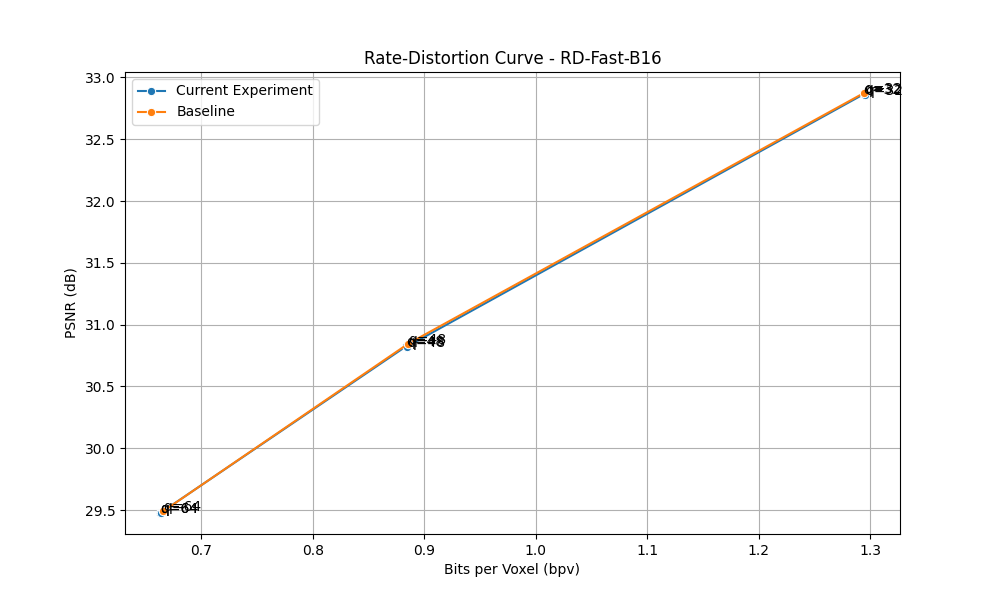
\includegraphics[width=\columnwidth]{images/B16/rd_curve.png}
    \caption{Curva tasa-distorsión para bloques de tamaño B16.}
    \label{fig:rd_b16}
\end{figure}

Para bloques B16, operando entre 0.66 y 1.30 BPV, RD-Fast presenta diferencias de PSNR entre $-0.02$ dB y $-0.01$ dB. Las diferencias de BPV son muy pequeñas, variando entre $-0.41\%$ y $+0.06\%$, lo que indica un desempeño prácticamente idéntico entre ambos métodos para este tamaño de bloque. Los bloques grandes reducen la capacidad de adaptación local pero disminuyen el overhead de señalización de modos.

\subsection{Análisis Comparativo}
El enfoque RD-Fast logra un rendimiento tasa-distorsión muy similar al método Baseline en todos los tamaños de bloque evaluados, con diferencias en PSNR típicamente dentro de $\pm 0.05$ dB. Las optimizaciones implementadas en RD-Fast, incluyendo la reducción del número de clusters de 4 a 2 y los ajustes en los parámetros de Simulated Annealing, no comprometen la calidad ni la tasa de compresión.

Un hallazgo importante es que la configuración con 2 clusters resulta suficiente para lograr un desempeño competitivo. La simplificación del modelo reduce la complejidad computacional sin sacrificar eficiencia de compresión, validando la hipótesis de que un único modo dinámico bien optimizado puede capturar las características relevantes de la señal.

La diferencia más notable se observa en bloques pequeños (B4), donde la ventaja en BPV es más pronunciada, mientras que para bloques grandes (B16) el desempeño converge al del método de referencia. La configuración simplificada ofrece ventajas prácticas: menor complejidad computacional en la fase de agrupamiento, menor overhead en la señalización de modos, y convergencia más rápida del algoritmo.

\section{Conclusiones}
Este trabajo presentó un método de compresión para nubes de puntos 3D basado en la Transformada de Fourier sobre Grafos (GFT) con un algoritmo de agrupamiento optimizado mediante criterios de Tasa-Distorsión. Los experimentos realizados evaluaron el desempeño del método propuesto (RD-Fast) en diferentes tamaños de bloque, comparándolo con un método de referencia (Baseline).

Los resultados demuestran que RD-Fast logra un rendimiento tasa-distorsión comparable al Baseline, con diferencias de PSNR típicamente dentro de $\pm 0.05$ dB. En varios casos, particularmente para bloques pequeños (B4), RD-Fast muestra mejoras modestas en eficiencia de bits, con reducciones de BPV de hasta $-1.01\%$. Esta equivalencia de desempeño, combinada con la configuración simplificada de 2 clusters, hace de RD-Fast una alternativa viable y práctica para aplicaciones de compresión de nubes de puntos.

Un hallazgo clave es que un único modo dinámico bien optimizado es suficiente para capturar las características relevantes de la señal en la nube de puntos evaluada. La configuración con 2 clusters ofrece ventajas prácticas significativas en términos de complejidad computacional y convergencia del algoritmo. Los parámetros de Simulated Annealing (temperatura inicial 1.0, temperatura final 0.1, tasa de enfriamiento 0.8) resultaron efectivos para explorar el espacio de soluciones evitando mínimos locales.

El impacto del tamaño de bloque sigue un patrón esperado: bloques pequeños (B4) permiten mayor adaptabilidad local y muestran las mayores ventajas de RD-Fast, bloques medianos (B8) ofrecen un compromiso óptimo entre adaptación y overhead, y bloques grandes (B16) convergen al desempeño del método de referencia debido a la reducción en granularidad de adaptación.

Trabajos futuros podrían explorar la aplicación del método a diferentes secuencias de nubes de puntos con características variadas, la evaluación de esquemas adaptativos que ajusten dinámicamente el número de clusters según las características locales de la señal, y estrategias de paralelización del algoritmo para mejorar su viabilidad en aplicaciones de tiempo real.

\bibliographystyle{IEEEtran}
\bibliography{references}
\end{document}